\documentclass[12pt,twoside]{article}
\usepackage[inner=1in,outer=0.6in,top=0.7in,bottom=1in]{geometry}
\usepackage{xeCJK}
\setmainfont{Times New Roman}
\setsansfont{Verdana}
\setmonofont{Courier New}                    % tt
\setCJKmainfont{微軟正黑體}
\setCJKfamilyfont{kai}{標楷體}		% for changing the title font in title.pgf -> have to manually 
\usepackage{graphicx}
\usepackage{pgf}
\usepackage{pstricks,pst-node}

\renewcommand{\today}{西元\number \year 年\ifcase \month \or 1月\or 2月\or 3月\or 4月\or 5月\or 6月\or 7月\or 8月\or 9月\or 10月\or 11月\or 12月\fi
} 

\begin{document}

\begin{pspicture}(0cm,0in)(6.5in,4in)
%\psgrid

\rput[br](6.5in,0cm){
\rnode{name}{
\large 東寧軟咖
}}

\rput[br](6.5in,0.6cm){
\rnode{time}{
\large \today
}}

\rput[bl](0cm,3.1cm){
\rnode{logo}{
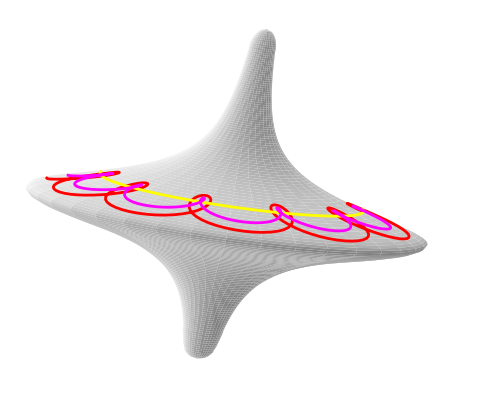
\includegraphics[scale=0.37]{../../figs/logo_June27_2016.png}
%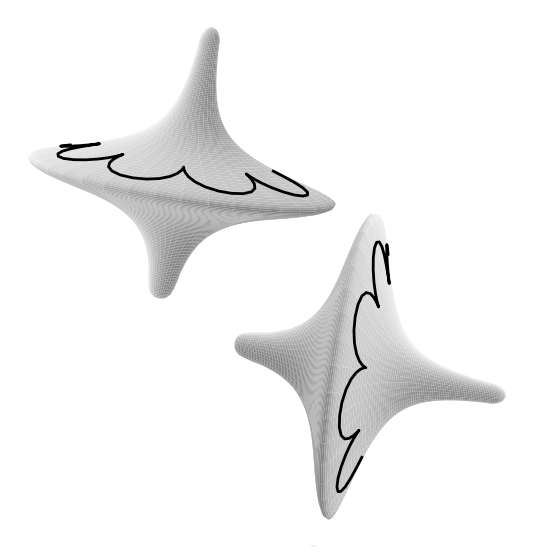
\includegraphics[scale=0.37]{./otherstuff/logo_Aug29_test.PNG}
}}

\rput[br](6.5in,7cm){
\rnode{title}{
\Huge 陀螺\hspace{0.8cm},方向追蹤,計算機轉動模擬器
%從陀螺聊到姿態追蹤與\\
%物理模擬引擎
%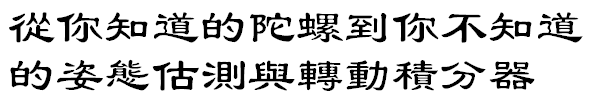
\includegraphics[scale=0.6]{./otherstuff/gyro_title_line4.PNG}%./otherstuff/
}}
%\psline(-0.8cm,0.4cm)(12.3cm,0.4cm)
\psline(0cm,3cm)(6.5in,3cm)

\rput[br](6.5in,1.4cm){
\rnode{running_title}{
\large \textcolor{gray}{
\parbox{10cm}{從基礎的貼體角速度與牛頓尤拉方程應用到\\姿態追蹤與電腦的轉動積分器,實作與應用。}
}
}}

\rput[br](6.5in,3.1cm){
\rnode{website}{
whymrandersonwhy.pythonanywhere.com
}}

\rput[br](6.5in,3.5cm){
\rnode{gss}{
\large \textcolor{gray}{GyroSoft Simulation}
}}

%\rput[B](5.5 cm,3.3cm){
%\rnode{E}{
%%\includegraphics[scale=0.5]{./decoration_line.PNG}
%\includegraphics[scale=0.5]{./otherstuff/decoration_line.PNG}
%}}





\end{pspicture}


\end{document}